\documentclass{beamer}

\usepackage{graphicx}
\usepackage{lmodern}
\usepackage[T1]{fontenc}
\usepackage{listings}
\lstset{columns=fullflexible}
\graphicspath{{./figures/}}

\title{Simple Machine Learning in Python using TensorFlow with Keras}
\author{Hunter Damron}
\date{Wednesday, October 2, 2019}
\institute[UofSC ACM]{Association for Computing Machinery -- University of South Carolina}

\setlength{\parskip}{\baselineskip}
\setlength{\parindent}{0pt}
\newcommand{\blue}[1]{\color{blue}{#1}}

\begin{document}
	\maketitle

	\begin{frame}{Overview}
		\begin{enumerate}
			\item Background and brief description of neural networks
			\item Implementation using Keras with TensorFlow
			\item Various demonstrations
			\item Why should I care?
		\end{enumerate}
	\end{frame}

	\begin{frame}{Welcome}
		This talk is intended to give a beginner-friendly introduction to machine learning using Python and the Keras/TensorFlow library. Neural networks have been successful in many different types of problems recently, from image recognition to board game strategy. Although the theory behind machine learning is complex, the Keras library makes it very easy to set up a simple neural network. We will be working in Python, but no experience is necessary to follow along. We look forward to seeing you, and we invite you to bring a friend from outside the department!

		The slides can be found \href{https://github.com/hdamron17/ACM_Machine_Learning_Talk/releases/}{\blue{here}}.
	\end{frame}

	\begin{frame}{Installation}
		\begin{enumerate}
			\item Ensure Python (preferably version 3.x) and \lstinline|pip| are installed
			\item Install Tensorflow: \lstinline|pip install tensorflow|
			\item Ensure you can import TensorFlow without errors: \lstinline|python -c "import tensorflow"|
		\end{enumerate}
	\end{frame}

	\begin{frame}{Successes of Neural Networks}
	\begin{itemize}
		\item DeepMind's \href{https://deepmind.com/research/case-studies/alphago-the-story-so-far}{\blue{AlphaGo}}
		\item Search engine recommendations
		\item Semantic image labeling
		\item Stock market prediction
		\item Medical diagnostics
		\item Etc. -- Neural networks are a very general tool
	\end{itemize}
	\begin{figure}
		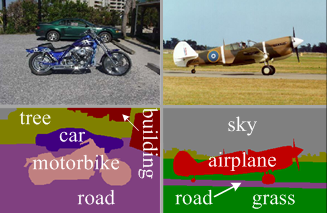
\includegraphics[width=0.65\textwidth]{semantic_labels}
	\end{figure}
	\end{frame}

	\begin{frame}{Background -- Neural Network}
	\begin{columns}
	\begin{column}{0.6\textwidth}
	\begin{itemize}
		\item Just a composition of many simple functions
		\item Capable of approximating any function if large enough
		\begin{itemize}
			\item Likely not the most concise approximation in many cases, though
		\end{itemize}
		\item Each layer (vertical in picture) transforms the data based on certain weights (from training) until the last layer gives an output
		\item Depth of a neural network is the number of layers
		\item Each node is called a ``neuron''
	\end{itemize}
	\end{column}
	\begin{column}{0.4\textwidth}
	\begin{figure}
		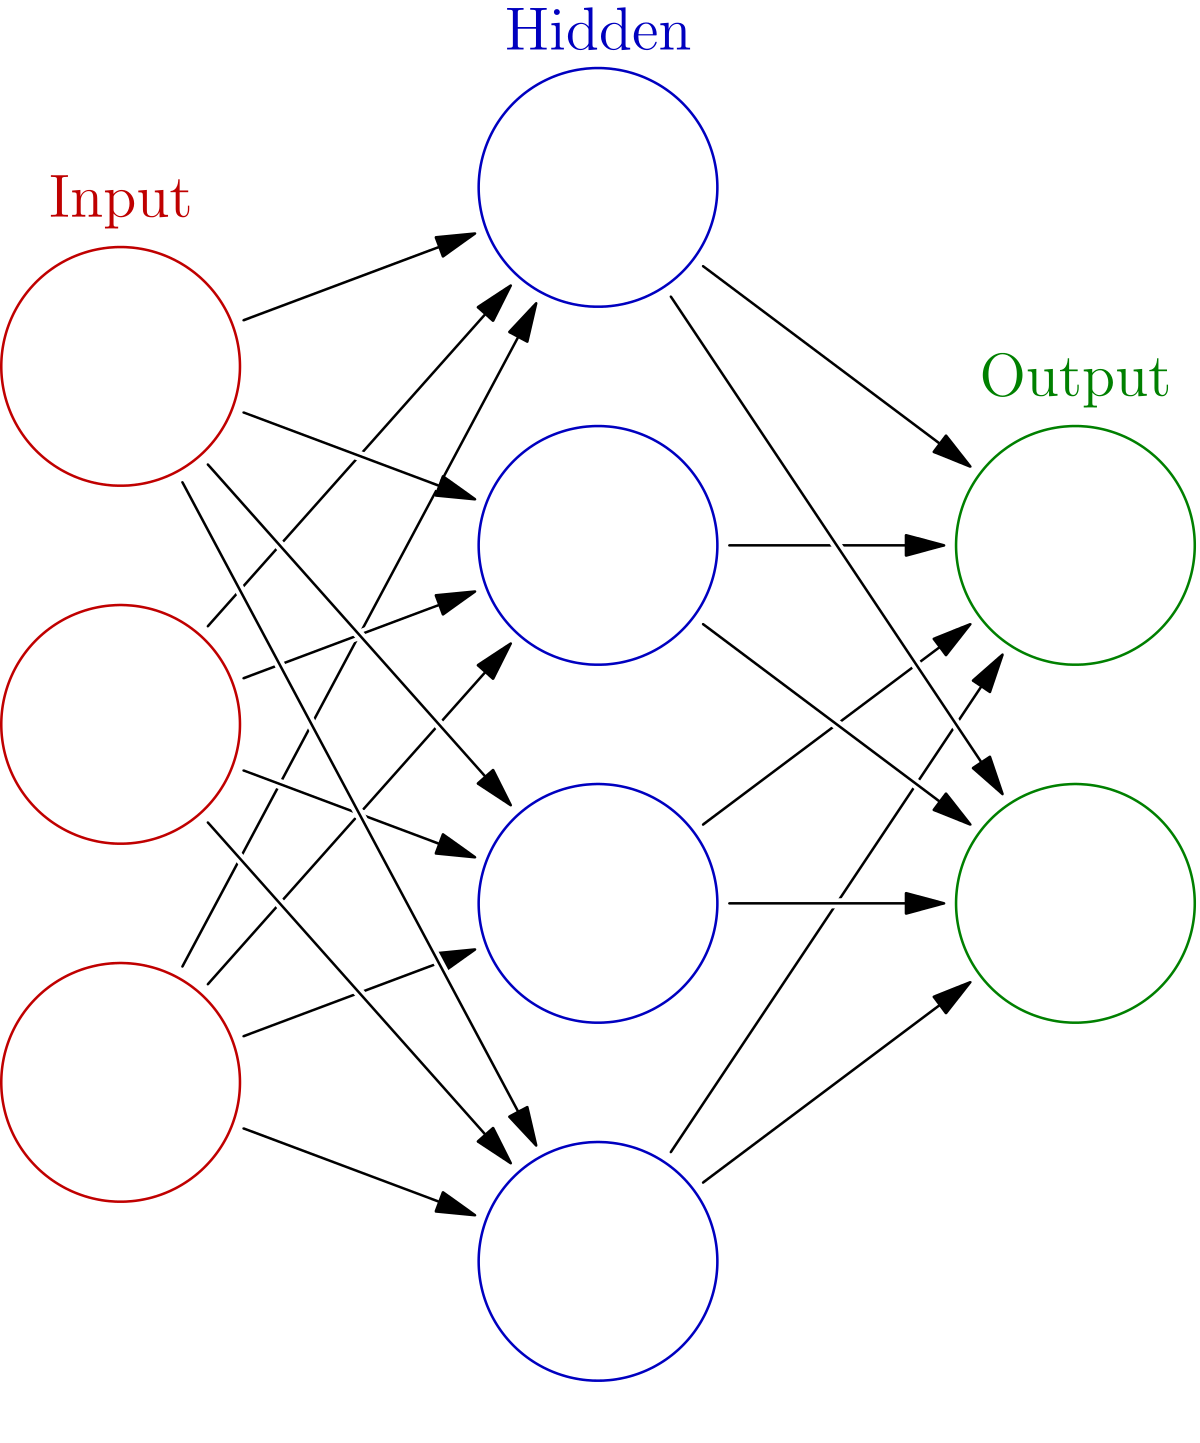
\includegraphics[width=\textwidth]{neural_network}
	\end{figure}
	\end{column}
	\end{columns}
	\end{frame}

	\begin{frame}{Background -- Neurons}
	\begin{itemize}
		\item Computes a weighted sum of its inputs with a bias
		\item Wraps this value in a nonlinear activation function
		\item Modeled on neurons in the brain
	\end{itemize}
	\begin{figure}
		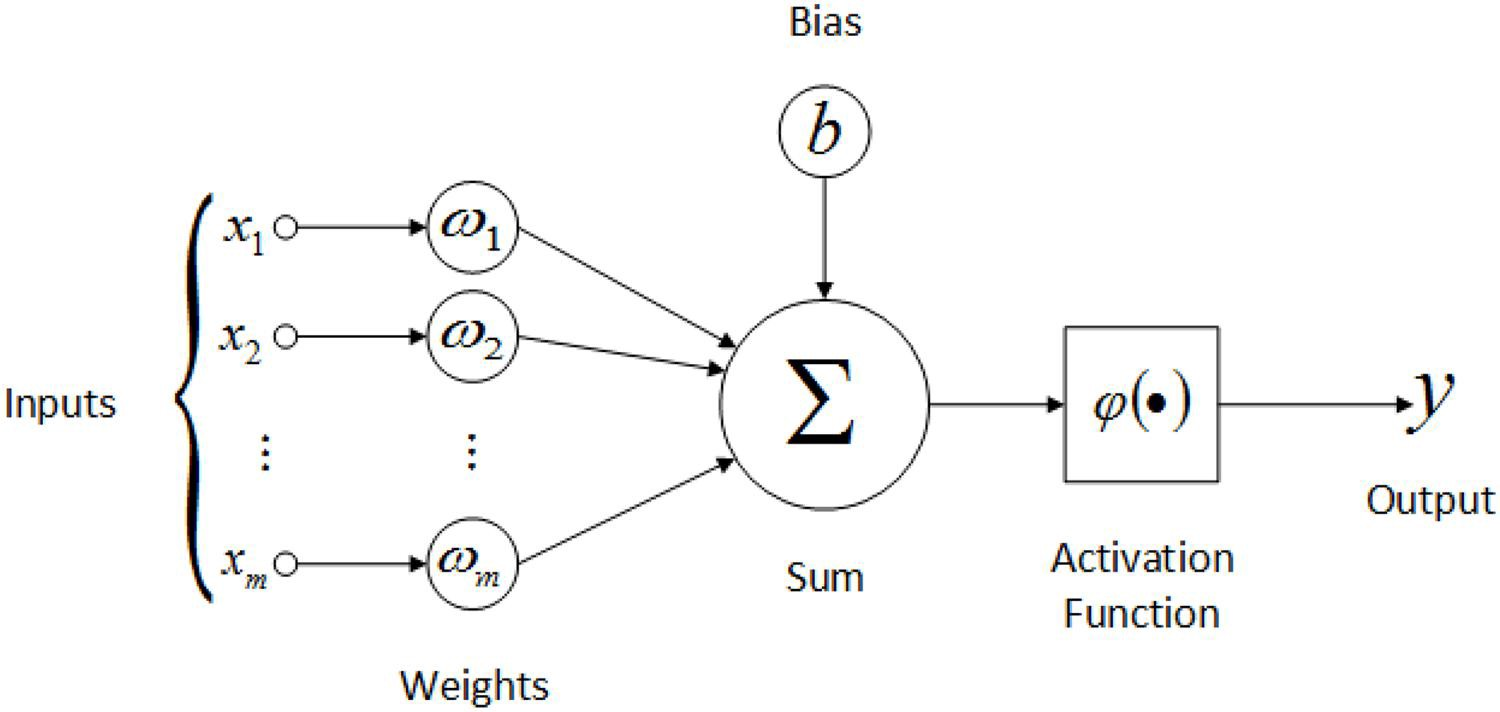
\includegraphics[width=0.7\textwidth]{neuron}
	\end{figure}
	\end{frame}

	\begin{frame}{Background -- Training}
	\begin{columns}
	\begin{column}{0.5\textwidth}
	\begin{itemize}
		\item Requires dataset with input data and the corresponding outputs
		\item Compares current approximation to known outputs and changes weights/biases of each neuron appropriately to reduce this error
		\item (Insert complex math here)
		\item Luckily, we can use a neural neural network library to do the hard work for us
	\end{itemize}
	\end{column}
	\begin{column}{0.5\textwidth}
	\begin{figure}
		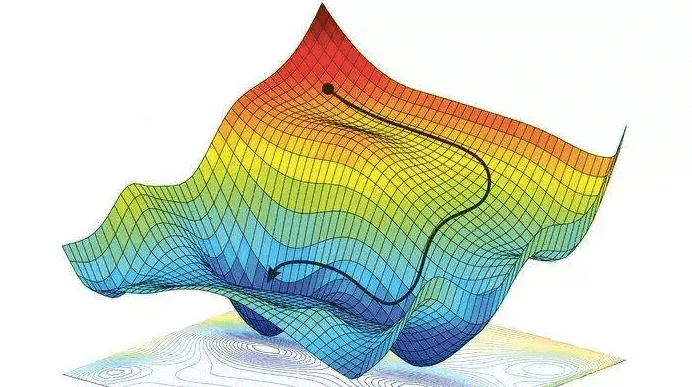
\includegraphics[width=\textwidth]{gradient_descent}
	\end{figure}
	\end{column}
	\end{columns}
	\end{frame}

	\begin{frame}{Background -- Evaluation Metrics}
	\begin{itemize}
		\item Loss (also error or loss) is used in training as a measure of how wrong the network currently is
		\begin{itemize}
			\item This choice is up to the designer
			\item Often Euclidean distance (possibly squared)
		\end{itemize}
		\item Accuracy (for classification) is the percentage of images properly classified
		\begin{itemize}
			\item Dataset usually split into training and testing datasets
			\item Testing on a different dataset ensures results are generalized
		\end{itemize}
		\item Root mean square error (RMSE) for regression type problems (answers can be partially correct)
	\end{itemize}
	\end{frame}

	\begin{frame}{Background -- Convolution for image recognition (CNN)}
	\begin{columns}
	\begin{column}{0.75\textwidth}
	\begin{itemize}
		\item A small pattern (or kernel) is used to detect a specific feature of the image
		\item Network learns kernel weights instead of all fully connected weights
		\item Example: For a small $128 \times 128$ image, a fully connected layer would require $(128 \times 128)^2 = 268435456$ weights
	\end{itemize}
	\end{column}
	\begin{column}{0.25\textwidth}
	\begin{figure}
		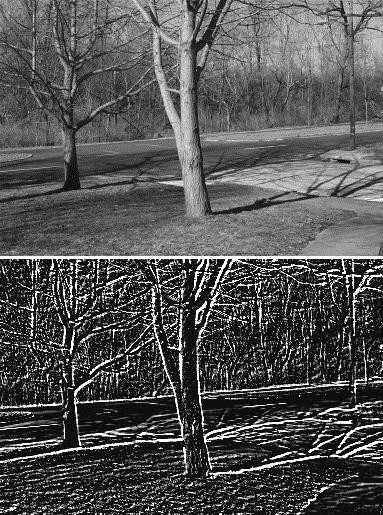
\includegraphics[width=\textwidth]{kernel}
	\end{figure}
	\end{column}
	\end{columns}
	\begin{figure}
		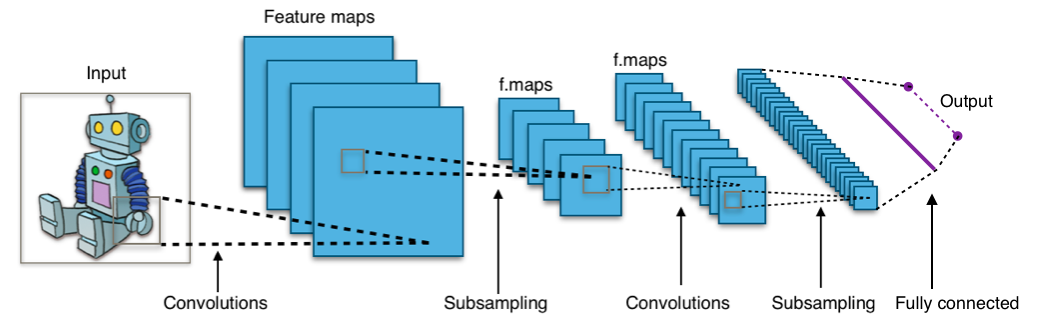
\includegraphics[width=0.9\textwidth]{cnn}
	\end{figure}
	\end{frame}

	\begin{frame}{TensorFlow and Keras}
	\begin{itemize}
		\item TensorFlow
		\begin{itemize}
			\item Free and open-source library by Google
			\item Symbolic computing with a focus on machine learning
			\item Speed boost using multiple CPUs and GPUs
			\item Works well with NumPy\footnote{NumPy is a godsend} data
		\end{itemize}
		\item Keras
		\begin{itemize}
			\item Free and open-source neural network library in Python
			\item Several backends, primarily TensorFlow
			\item Handles all the complex math for you
		\end{itemize}
	\end{itemize}
	\end{frame}

	\begin{frame}{Common Keras Layers}
	\begin{itemize}
		\item Dense (Fully Connected)
		\begin{itemize}
			\item Customized by activation function
		\end{itemize}
		\item Conv2D
		\begin{itemize}
			\item For spatially related data (e.g.\ images and time series)
			\item Customized by kernel size
		\end{itemize}
		\item Pooling (Max, Min, Average)
		\begin{itemize}
			\item For downsizing data
			\item Customized by pool size
		\end{itemize}
		\item Dropout
		\begin{itemize}
			\item For preventing overfitting
			\item Customized by dropout rate
		\end{itemize}
	\end{itemize}
	\end{frame}

	\begin{frame}{Common Keras Activation Functions}
	\begin{columns}
	\begin{column}{0.5\textwidth}
	\begin{itemize}
		\setlength{\abovedisplayskip}{1ex}
		\setlength{\belowdisplayskip}{1ex}
		\item Rectified Linear Unit (ReLU)
		\[ ReLU(x) =
		\begin{cases}
		x & \text{ if } x \geq 0 \\
		0 & \text{ else}
		\end{cases} \]
		\item Hyperbolic tangent (tanh)
		\[ \tanh(x) = \frac{e^x - e^{-x}}{e^x + e^{-x}} \]
		\item Logistic sigmoid
		\[ S(x) = \frac{1}{1 + e^{-x}} \]
		\item Softmax
		\[ \sigma(\vec{x})_i = \frac{e^{\vec{x}_i}}{\sum_{j=1}^n e^{\vec{x}_i}} \text{ for } \vec{x} \in \mathbb{R}^n \]
		\item Others listed \href{https://keras.io/activations/}{\blue{here}}
	\end{itemize}
	\end{column}
	\begin{column}{0.5\textwidth}
		\begin{figure}
			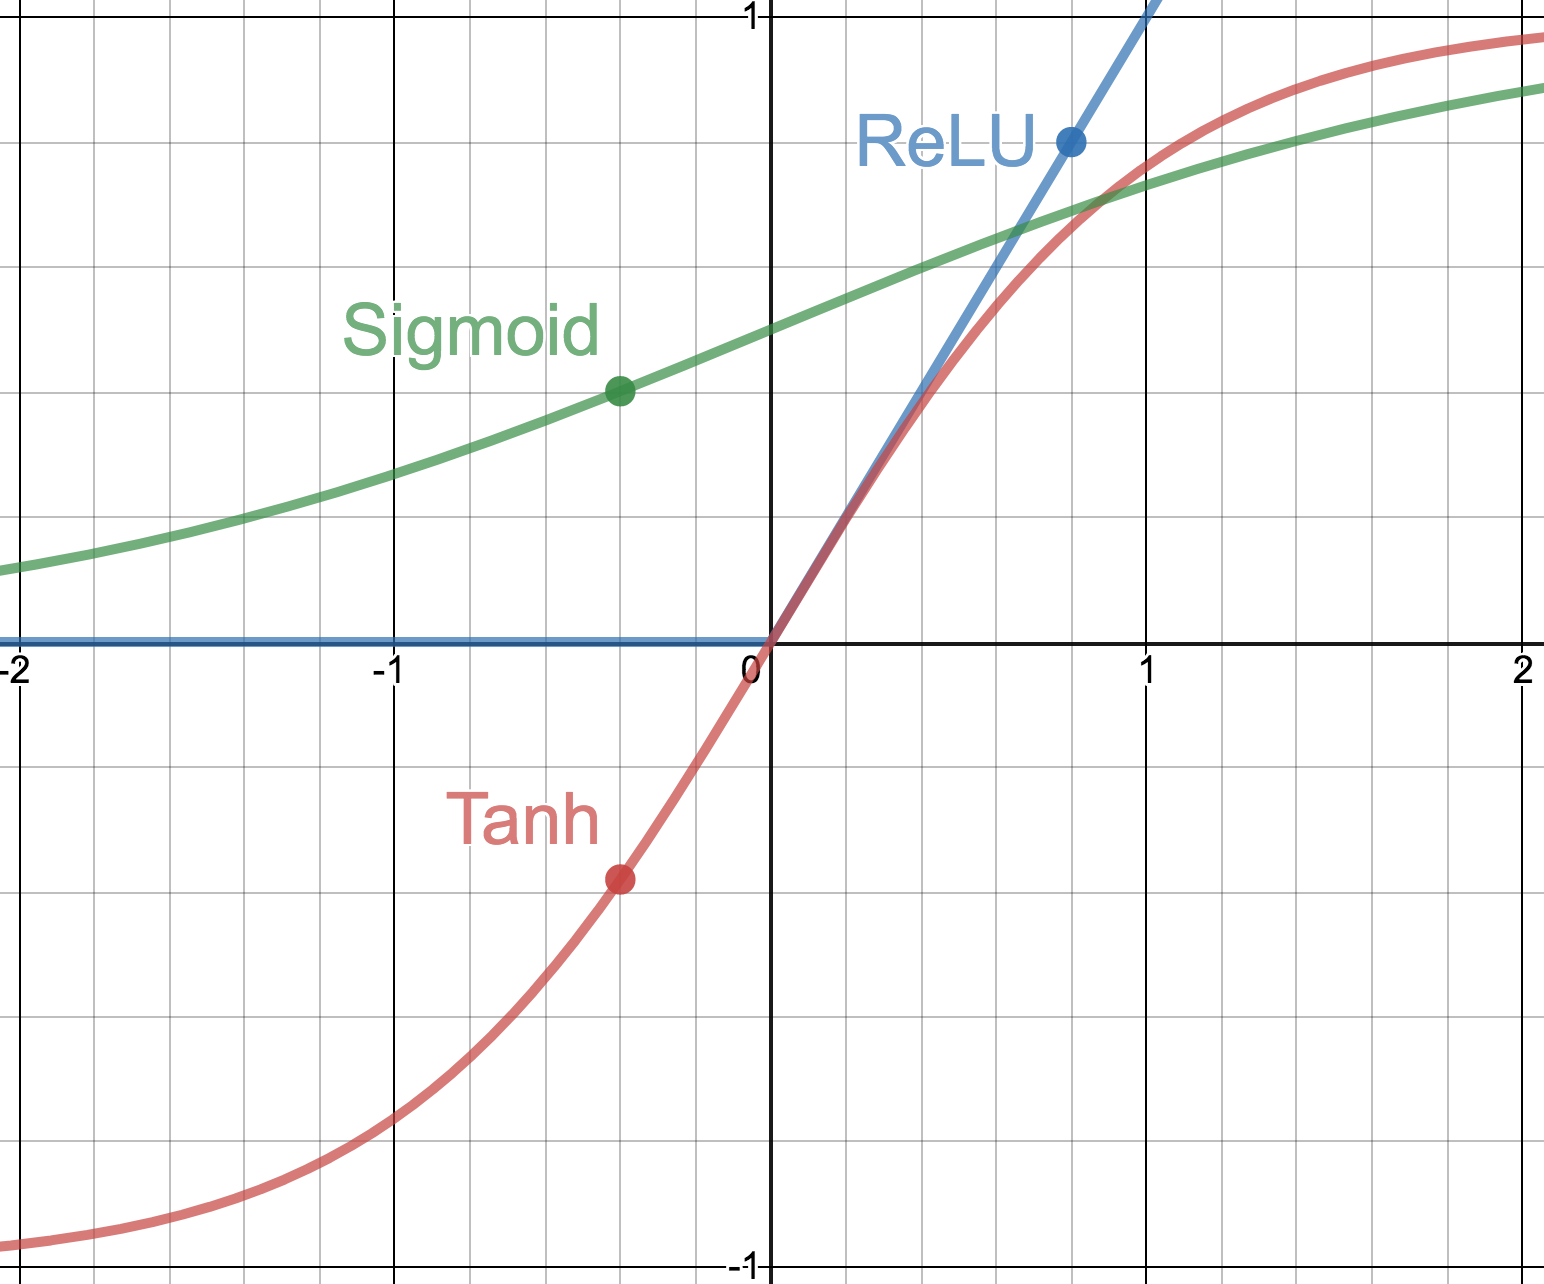
\includegraphics[width=\textwidth]{activations}
		\end{figure}
		\begin{center}
		(Created using \href{https://www.desmos.com/calculator}{\blue{Desmos}})
		\end{center}
	\end{column}
	\end{columns}
	\end{frame}

	\begin{frame}{MNIST Handwriting Recognition}
	\begin{columns}
	\begin{column}{0.7\textwidth}
	\begin{itemize}
		\item The \href{http://yann.lecun.com/exdb/mnist/}{\blue{MNIST dataset}} is commonly used for evaluating machine learning techniques
		\item Thousands of handwritten digits
		\item Built into keras using \lstinline|tf.keras.datasets.mnist.load_data()|
		\item Keras sample code \href{https://www.tensorflow.org/tutorials/quickstart/beginner}{\blue{here}} (we will use my \href{https://colab.research.google.com/drive/170ejXXwx5x_0gOyYo_3KaOu-NwLzHaA5}{\blue{modified version}} which includes extra demonstration)
		\item Another sample code for clothing image classification \href{https://www.tensorflow.org/tutorials/keras/classification}{\blue{here}} (we will again use my \href{https://colab.research.google.com/drive/1JPLrS8sYrfCCWXRtW5xDcgqFJoVAfhdJ}{\blue{modified version}} which uses a CNN)
	\end{itemize}
	\end{column}
	\begin{column}{0.3\textwidth}
		\begin{figure}
			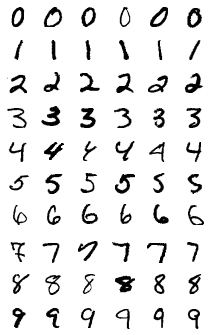
\includegraphics[width=\textwidth]{mnist}
		\end{figure}
	\end{column}
	\end{columns}
	\end{frame}

	\begin{frame}{TensorFlow Playground}
		\begin{figure}
			\href{https://playground.tensorflow.org/}{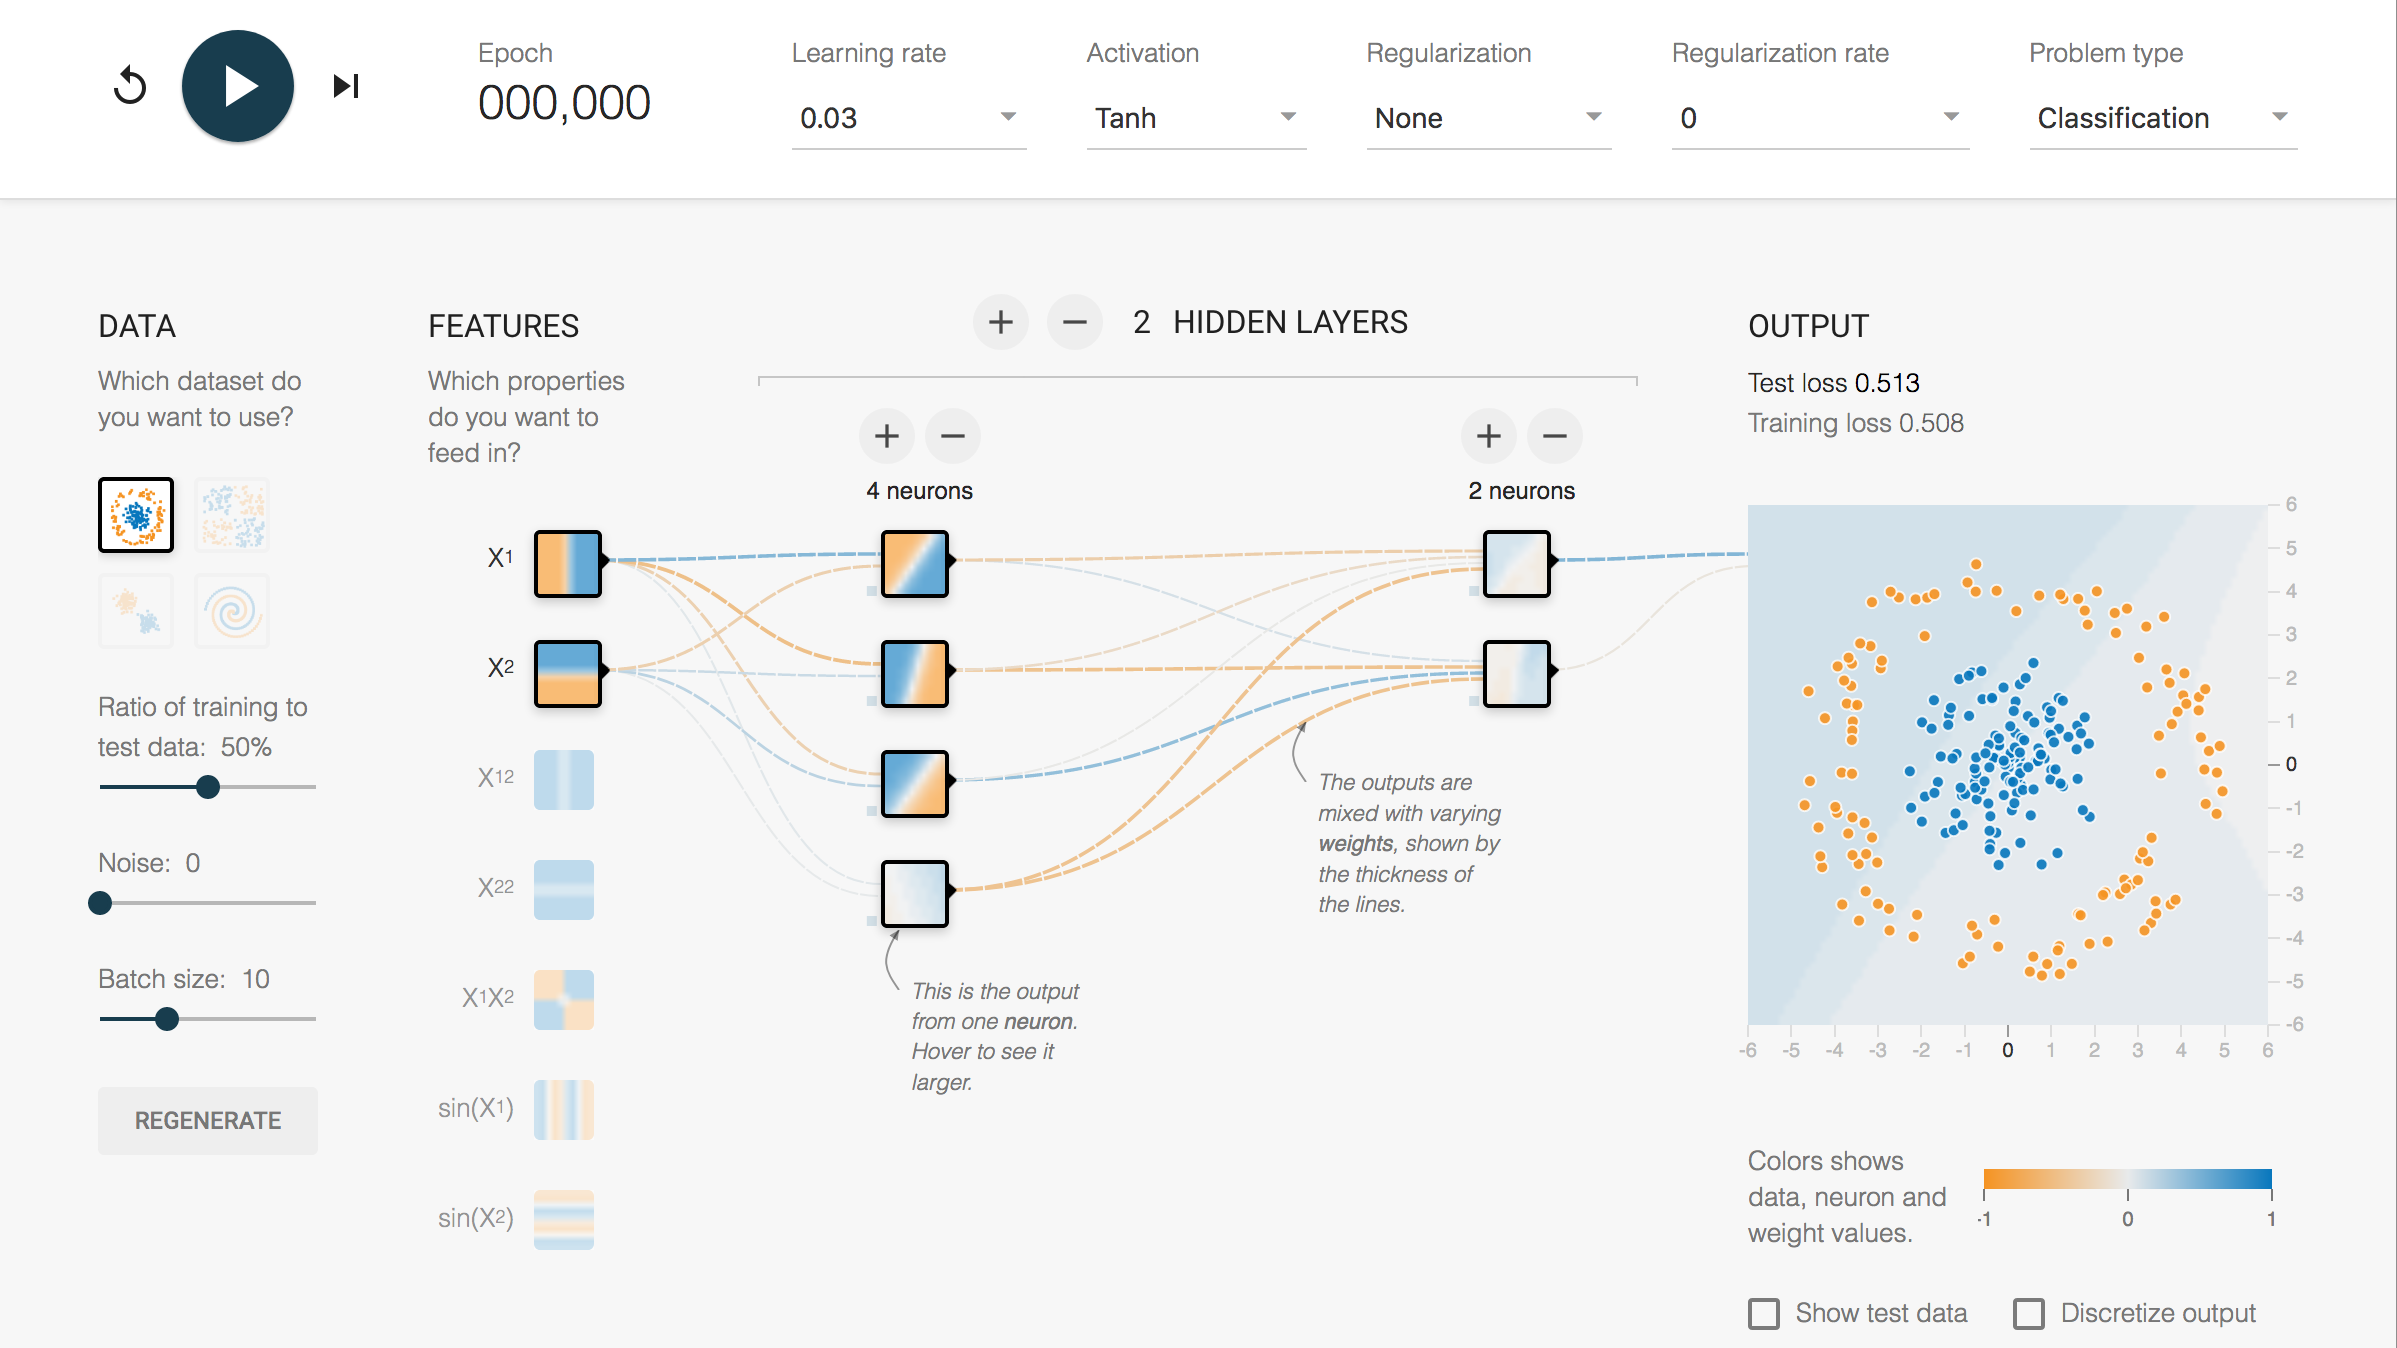
\includegraphics[width=\textwidth]{playground}}
		\end{figure}
		Try it \href{https://playground.tensorflow.org/}{\blue{here}}.
	\end{frame}

	\begin{frame}{What does this mean for me?}
	\begin{itemize}
		\item You can recognize handwritten digits (yeah, I already could)
		\item More importantly, you now understand how one of the most popular algorithms of the millennium works
		\item You understand why everyone seems to be trying to collect data about everything you do
		\item You understand why the abundance of Python packages make it so enticing
	\end{itemize}
	\end{frame}

	\begin{frame}{Additional Resources}
	\begin{itemize}
		\item Many good \href{https://www.tensorflow.org/tutorials}{\blue{tutorials}} for programmers of all experience levels (one is the basis of this talk)
		\item Keras \href{https://keras.io/}{\blue{documentation}} provides information about how to use Keras layers and gives sample codes
		\begin{itemize}
			\item Note that you can replace `\lstinline|keras|' with `\lstinline|tf.keras|' in these samples to avoid installing another package
		\end{itemize}
	\end{itemize}
	\end{frame}
\end{document}